\documentclass{article}
\usepackage{tikz}
\usepackage{pgfplots}
\usepackage{xcolor}

% 定义颜色

\definecolor{my1}{RGB}{142,207,201}
\definecolor{my2}{RGB}{255,190,122}
\definecolor{my3}{RGB}{35,186,197}
\definecolor{my4}{RGB}{130,176,210}

\definecolor{my5}{RGB}{255,230,200} % 更浅的橙色
\definecolor{my6}{RGB}{175,240,245} % 更浅的蓝色


% 导入必要的库
\usepackage{amssymb}
\usetikzlibrary{shapes.geometric}
\usetikzlibrary{arrows,decorations.pathmorphing,backgrounds,positioning,fit,petri}
\usetikzlibrary{arrows.meta,fit,shapes.arrows}
\usepackage{caption}
\usepackage{subfig}
\usetikzlibrary{positioning,shapes,arrows,shadows,patterns}
\usetikzlibrary{calc}

% 设置pgfplots参数
\pgfplotsset{
    width=0.82\textwidth, % 图表宽度
    height=0.3\textheight, % 图表高度
    grid=major, % 显示主网格
    major grid style={dotted}, % 主网格样式
    symbolic x coords={WMT22,IWSLT17}, % x轴标签
    legend style={
        at={(0.5,0.95)}, % 图例位置
        anchor=north, % 图例锚点
        legend columns=2 % 图例列数
    },
}

% 设置图例与下文的间距
\captionsetup{belowskip=-10pt}

\begin{document}
\begin{figure}[!t]
  \centering
  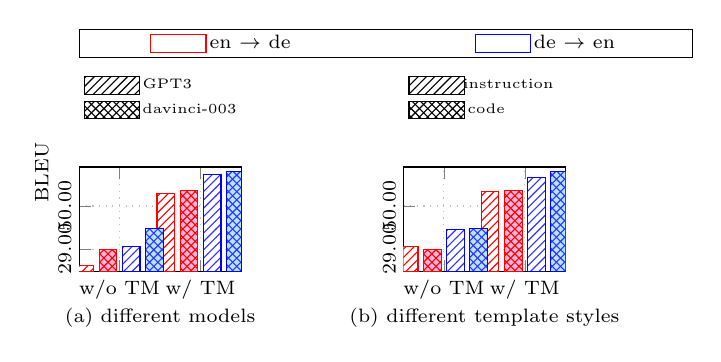
\begin{tikzpicture}
  \centering
  % \sisetup{round-precision = 2}
  % \tikzstyle{modelnode} = [rectangle,draw=red,rounded corners=2pt,inner sep=2pt,minimum height=1em,minimum width=2em,font=\small,anchor=north]
    \scriptsize{
    \begin{axis}[
      at={(0,0)},
      ymajorgrids,
      grid style=dashed,
      legend style={at={(0.41,0.54)}, anchor=south west},
      legend cell align={left},
      ybar,
      enlarge x limits=0.5,
      xtick align=inside,
      height=.24\textwidth,
      width=.30\textwidth,
      bar width=0.8em,
      xlabel={(a) different models},
      % ylabel={BLEU},
      symbolic x coords={w/o TM,w/ TM},
      legend style={cells={align=left}},
      xtick=data,
      %nodes near coords,
      nodes near coords align={vertical},
      ymin=18.00,
      ymax=69.00,
      ytick={29.00,50.00},
      xticklabels={w/o TM,w/ TM},
      %x tick label style={
      %      rotate=45,
      %      anchor=east,
      %  },
      %enlarge x limits=0.1,
    %   enlarge y limits=0.3,
      ylabel style={yshift=-3em},xlabel style={yshift=0.3em,align=center},
      yticklabel style={/pgf/number format/fixed,/pgf/number format/fixed zerofill,/pgf/number format/precision=2,rotate=90},
      legend style={draw=none,
        line width=1pt,
        at={(0.5,1.0)},
        anchor=south},
        xtick=data,
      ]
          % en2de GPT3
         \addplot[fill=white,draw=red, area legend,postaction={pattern=north 
east lines},pattern color=red] coordinates {(w/o TM,20.91) (w/ TM,56.13) };
          % en2de davinci-003
          \addplot[ fill=magenta!30,draw=red, area legend,postaction={pattern=crosshatch},pattern color=red] coordinates {(w/o TM,29.00) (w/ TM,57.39) };

          % de2en GPT3
          \addplot[fill=white, draw=blue, area legend,postaction={pattern=north 
east lines},pattern color=blue!80] coordinates {(w/o TM,30.31) (w/ TM,65.48) };
% \addlegendentry{de→\rightarrowen GPT3};
          % de2en davinci-003
          \addplot[fill=cyan!30, draw=blue, area legend,postaction={pattern=crosshatch },pattern color=blue!80] coordinates {(w/o TM,38.89) (w/ TM,66.90) };
          % \addlegendentry{de→\rightarrowen davinci-003};
    \end{axis}
    } 
    \node [rectangle,draw=black,inner sep=2pt,minimum height=0.8em,minimum width=2.5em,font=\small,anchor=north,align=center,pattern=north east lines] (label1) at (1.5em,8.85em){};
    \node [rectangle,draw=black,inner sep=2pt,minimum height=0.8em,minimum width=2.5em,font=\small,anchor=north,align=center,pattern=crosshatch] (label2) at (1.5em,7.75em){};
    \node [align=center] (label1_1) at ([xshift=2.5em,yshift=-0.35em]label1.north){\tiny GPT3};
    \node [rectangle,draw=red,inner sep=2pt,minimum height=0.8em,minimum width=2.5em,font=\small,anchor=north,align=center] (a) at (4.5em,10.77em){};
    \node [align=center] (label1_2) at ([xshift=3.5em,yshift=-0.35em]label2.north){\tiny davinci-003};
    % \node [align=center] (a1) at ([xshift=3.25em,yshift=-0.35em]a.north){en →\rightarrow de};
    \scriptsize{
    \begin{axis}[
      at={(14.7em,0)},
      ymajorgrids,
      %xmajorgrids,
      grid style=dashed,
      legend style={at={(0.02,0.65)}, anchor=south west},
      legend cell align={left},
      ybar,
      enlarge x limits=0.5,
      xtick align=inside,
      height=.24\textwidth,
      width=.30\textwidth,
      bar width=0.8em,
      xlabel={(b) different template styles},
      % ylabel={BLEU},
      symbolic x coords={w/o TM,w/ TM},
      legend style={cells={align=left}},
      xtick=data,
      %nodes near coords,
      nodes near coords align={vertical},
      ymin=18.00,
      ymax=69.00,
      ytick={29.00,50},
      xticklabels={w/o TM,w/ TM},
      ylabel style={yshift=-3em},xlabel style={yshift=0.3em,align=center},
      yticklabel style={/pgf/number format/fixed,/pgf/number format/fixed zerofill,/pgf/number format/precision=2,rotate=90},
      legend style={draw=none,
        line width=1pt,
        at={(0.5,1.0)},
        anchor=south},
        xtick=data,
      ]
          % en2de instruction
          \addplot[fill=white,draw=red, area legend,postaction={pattern=north 
east lines},pattern color=red] coordinates {(w/o TM,30.2) (w/ TM,56.88) };
          % en2de code
          \addplot[ fill=magenta!30,draw=red, area legend,postaction={pattern=crosshatch},pattern color=red] coordinates {(w/o TM,29.00) (w/ TM,57.39) };
          % de2en instruction
          \addplot[fill=white, draw=blue, area legend,postaction={pattern=north 
east lines},pattern color=blue!80] coordinates {(w/o TM,38.38) (w/ TM,63.97) };
% \addlegendentry{de$\rightarrow$en code-style};
          % de2en code
          \addplot[fill=cyan!30, draw=blue, area legend,postaction={pattern=crosshatch },pattern color=blue!80] coordinates {(w/o TM,38.89) (w/ TM,66.90) };
          % \addlegendentry{de$\rightarrow$en instruction-style};

    \end{axis}
    }
    \node [rectangle,draw=blue,inner sep=2pt,minimum height=0.8em,minimum width=2.5em,font=\small,anchor=north,align=center] (b) at (19.2em,10.77em){};
    
    \node [align=center] (b1) at ([xshift=3.25em,yshift=-0.35em]b.north){de $\rightarrow$ en};
    \node [rectangle,draw=black,inner sep=2pt,minimum height=1.25em,minimum width=27.8em,font=\small,anchor=north,align=center] (final) at (13.9em,11em){};

    \node [align=center] (a1) at ([xshift=3.25em,yshift=-0.35em]a.north){en $\rightarrow$ de};
        %%%%%%%%%%%%%%%%%%%%%%%%%%
    \node [rectangle,draw=black,inner sep=2pt,minimum height=0.8em,minimum width=2.5em,font=\small,anchor=north,align=center,pattern=north east lines] (label1) at (16.2em,8.85em){};
    \node [rectangle,draw=black,inner sep=2pt,minimum height=0.8em,minimum width=2.5em,font=\small,anchor=north,align=center,pattern=crosshatch] (label2) at (16.2em,7.75em){};
    \node [align=center] (label1_1) at ([xshift=3.25em,yshift=-0.35em]label1.north){\tiny instruction};
    \node [align=center] (label1_2) at ([xshift=2.25em,yshift=-0.35em]label2.north){\tiny code};
    \node [rotate=90]at (-1.7em,4.5em) {BLEU};

\end{tikzpicture}
  \caption{Comparison of COMET22 scores for different models on WMT22 and IWSLT2017 datasets} % 图标题
  \label{fig:data-comparison} % 图标签
\end{figure}
\end{document}
